\documentclass[conference]{IEEEtran}

\usepackage{cite}
\usepackage{amsmath,amssymb,amsfonts}
\usepackage{algorithmic}
\usepackage{graphicx}
\usepackage{textcomp}
\usepackage{xcolor}
\usepackage{times}
\usepackage{latexsym}
\usepackage[super]{nth}
\usepackage{url}

\title {Open Set Classification and Novelty Detection in Text and Vision }
\author{Suad Alhojely}

 
\begin{document}


\maketitle
\begin{abstract}
Text classification is a significant task in the area of text mining, and it is required more than ever due to the increase in using the data on the Internet. In last year, the researcher has been trying to find features that could help to create an accurate model in order to recognize the data for all classes in classification. In a given a set of class, recognize one class from the other classes, is classification that involves learning for a given document. Accurate classifier, which determines all known classes during training test, is called Close World. In contrast, unknown classes can be seen during training test time is the Open World. Open-set World is a classifier that not identified unseen classes during training to other classes, which lead to a lack of performance to the state-of-art classifier.  This survey presents the study of open classification for text and image. Also, it will explain the related topics for the open world such as Novelty Detection,  and Outlier detection. We explain methods of novelty detection. 

\end{abstract}


\section{Introduction}

\par A fundamental assumption made by supervised learning or text classification is that every class appears in the test data must have appeared in training data, this is called the closed-world assumption (Bendale & Boult, 2015; Scheirer et al., 2013; Fei & Liu, 2016; Chen & Liu, 2016). But open-world assumption classifies examples from the known classes that appeared during training and also reject examples from unseen classes that do not appear in training data.


A classifier is aware of what it does and does not know. Most classifiers use closed set domains. However, the common problem, falls into the open set category (Grudic,n.d.) \cite{grudicclassification}. Some text classification applications are sentiment analysis, spam
filtering and document classification \cite{prakhya2017open}.

\par Open text classification should be able to do this denomination. First is to assign every example to one of the known classes that appeared in training data, and reject those examples from unknown classes that do not appear in training. Second is to discover unknown classes in the rejected examples, and finally is to learn the new classes incrementally\cite{shu2018unseen}. Figure 1 illustrates the difference between closed and open sets (Scheirer et al., 2013)


\begin{figure}[h!]
\centering
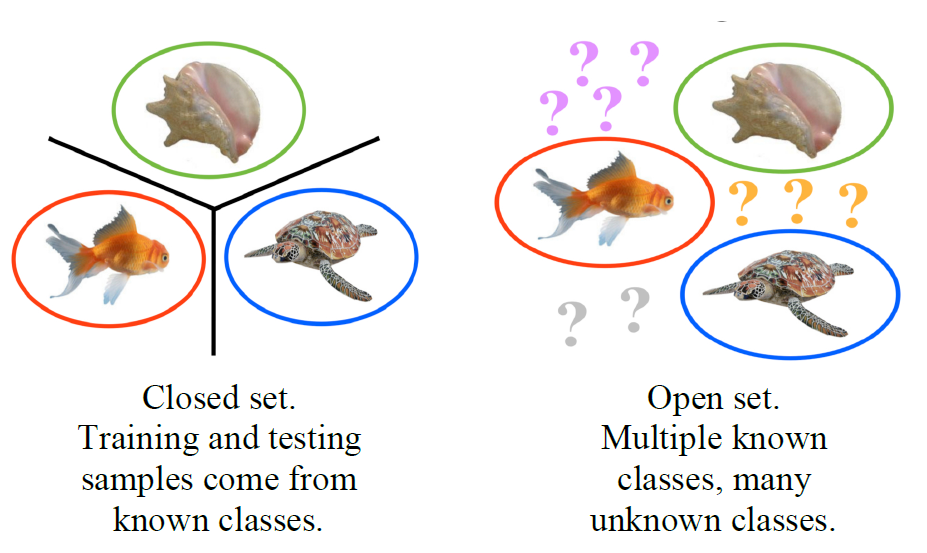
\includegraphics[width=0.4\textwidth]{soso.PNG}
\caption{\label{fig:Capture-suad} The difference between closed and open sets is that closed sets assume that all classes are seen during training, while open sets assume there are unknown classes not yet encountered during testing time.}
\end{figure}


\par Moreover, there are related topics to open set such as Novelty Detection and Outlier Detection. Many people would say Novelty Detection and Open-set Classification are the same, but others disagree. Novelty detection refers to the identification of unknown data that a machine learning system is not aware of during a training set. Abnormality detection indicates to problems of finding unknown data, and these unknown data refer to outliers or anomalies in many application domains such as fraud detection, military surveillance, and fault detection.  Anomalies or outliers are the most commonly used in the context of Novelty Detection interchangeably. Novelty Detection \cite{markou2003novelty} \cite{markou2003novelty} and Abnormality detection \cite{chandola2009anomaly} are related to each other. The difference between novel and anomalies patterns is that the novel is integrated into the normal pattern after being detected \cite{chandola2009anomaly}.

\par As early as the \nth{19} century, the outliers or anomalies detection has been elaborate in statistics communities \cite{edgeworth1887xli}. With time, many abnormality detection methods have developed in several application domains.


\par An abnormality is a pattern in data during training time that does not fit as part of expected behavior. For instance, Figure 2 shows that the sample of two-dimensional data with two common regions N1 and N2. While the other point o1, o2, and the points in O3   are far away from the regions, they are anomalies. \cite{chandola2009anomaly}.

\begin{figure}[h!]
\centering
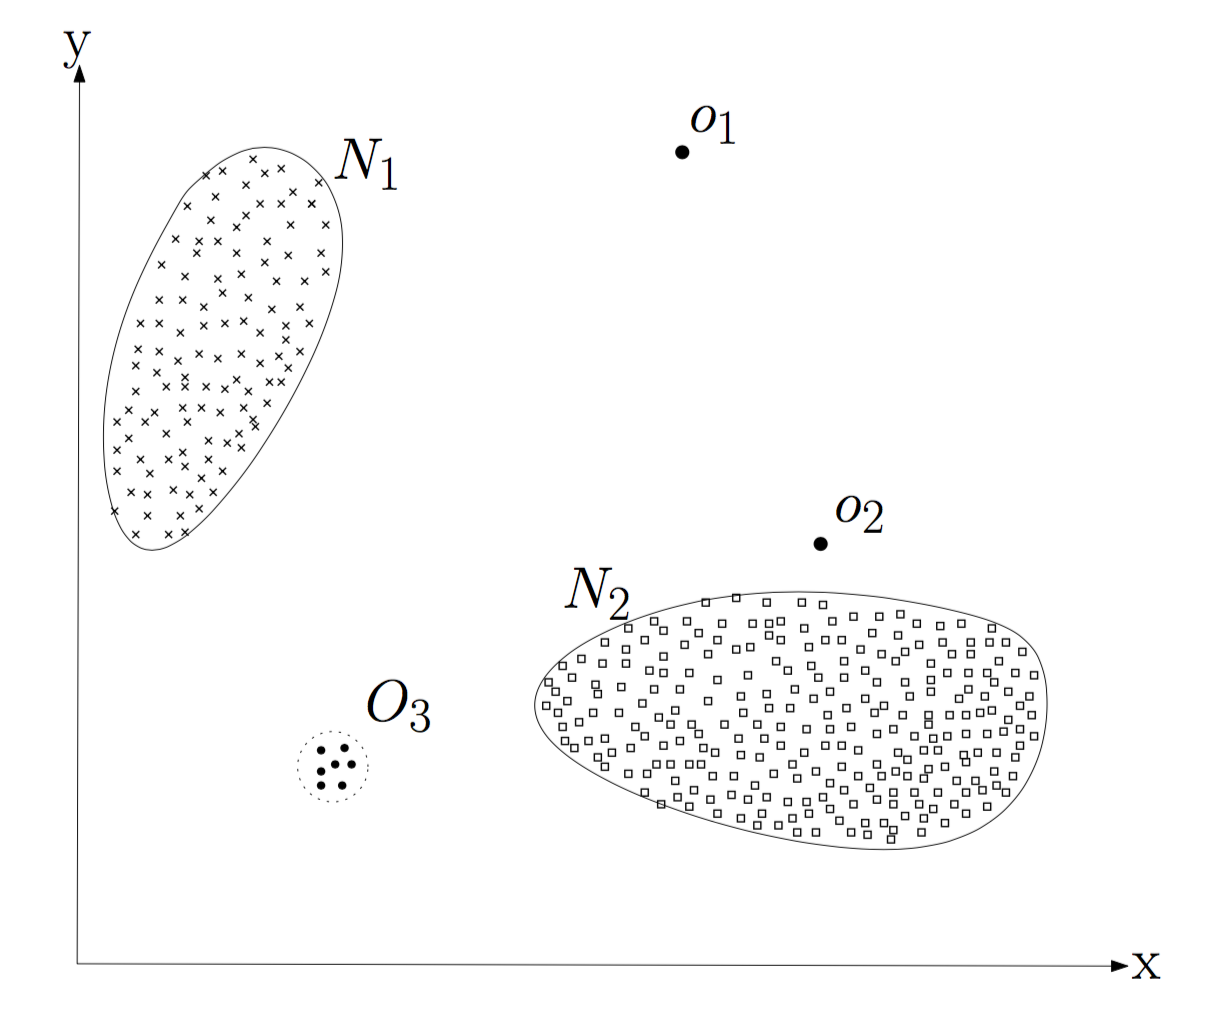
\includegraphics[width=0.3\textwidth]{11.png}
\caption{\label{fig:Capture-suad}   A sample example in a 2-dimensional data set of anomalies adopted by \cite{chandola2009anomaly}}
\end{figure}


% Anomaly detection is related to, but distinct from noise removal [Teng et al. 1990] and noise accommodation [Rousseeuw and Leroy 1987], both of which deal with unwanted noise in the data. Noise can be defined as a phenomenon in data which is not of interest to the analyst, but acts as a hindrance to data analysis. Noise removal is driven by the need to remove the unwanted objects before any data analysis is performed on the data. Noise accommodation refers to immunizing a statistical model estimation against anomalous observations [Huber 1974]. form this paper \cite{chandola2009anomaly}

The following sections show the content of the research about the open world classification and novelty detection. 

%problems like 
%new word
%miss spelling
%proper noun 9( names)

\section{Open Set Classification}

This section shows the open set classification related work in text and vision ordered by year. 

\subsection{ Open Set in Text:}


 \par Fei and Liu, in 2015 proposed a novel technique called Center Based Similarity (CBS), to solve the problem of covariate shift in classification. The key is the transformation of the original document from D-space with n-gram space to CBS space because the CBS learning in similarity space. The new space in the proposed technique of covariate shift problem is qualifying to build much better classifiers. The difference between D-space and CBS is document representation \cite{fei2015social}. However, that is suitable for open classification \cite{fei2016breaking}.  The problem of covariate shift in Machine Learning is a type of sample selection bias; additionally, they used Amazon review data-sets \cite{jindal2008opinion}.  (Fei and Liu, 2015) conclude that the proposed technique performed better than baseline such as SVM, and it improves classification\cite{fei2015social}.




% (Fei and Liu, 2016) 
\par The authors Fei and Liu in 2016 tried to solve the open-set problem by proposing CBS space learning strategy in order to decrease open space risk, and balance the empirical risk for open classification. The researcher proposed CBS space method which calculates a center for every class and then transforms every document to a vector in the center. After building the classifier by using transformed data, the surface is like a ball surrounding every class, but every class outside the ball becomes unknown \cite{fei2016breaking}. 

 
 \par They did an extensive experiment, and they used two data sets. The first data set is  20-newsgroups that contained 18828 documents. The second data set is  Amazon reviews that contained 50 types of products, and every product has 1000 reviews \cite{rennie200820} \cite{jindal2008opinion}. Their experiment shows that cbsSVM on multi-class open set text classification makes an excellent classifier compared to state-of-the-art methods. The solution for CBS learning reduces the positive label area from infinite space to finite space which significantly decreases open space risk. 
 
\par They explain that the proposed solution is hopeful, but they need to design a robust solution that works with the known class. The reason for the classifier is not informed enough to refuse unknown classes; this is because of significant open space risk in their proposed solution.




%(Tri and Jugal, 2017)

\par   The researchers Tri and Jugal  proposed Nearest Centroid Class classifier in 2017. Their goal of the classifier is to expose unknown classes incrementally. They test NCC on document classification on many domains, and they found promising results. They said that Random Forests is the promising model more than SVM because of RF ability to remove and add components \cite{doanbreaking}. 
The distance-based method such as  Nearest Class Mean (NCM) present each class by mean, and sphere shape of centered class locate to a boundary of a known class. Outside the sphere shape is an outlier on the unknown, in the open space. The logic of NCM inspires their proposed model. They designed a set of closest centroid class by using DBSCAN algorithm which clustered that represents one data point \cite{doanbreaking}. 



\par They use the same data sets presented in \cite{rennie200820} \cite{jindal2008opinion}. Their model performs well, and the gradual loss in performance as more as an unknown class shown in testing \cite{doanbreaking}. 



\par Shu et al.  propose a novel deep learning approach for open classification world in 2017, which perform better than existing state-of-the-art techniques. They proposed a method similar to CBS but were out-performed by Fei significantly better \cite{fei2016learning}. Fei et al.  added a capability of identifying new classes and incorporating them, which is essential because any system will not be able to learn by itself without the ability to learn and identify new aspects \cite{chen2016lifelong} \cite{fei2016learning}. 

\par Their proposed system is Deep Open Classification (DOC) which uses deep learning. To decrease open space risk, they use the 1-vs-rest final layer of sigmoid with the multi-class classifier. DOC uses CNN because it performs well in text \cite{kim2014convolutional}. They used the same data sets used in \cite{fei2016breaking} \cite{rennie200820} \cite{chen2014mining}. However, they compared DOC with two state-of-the-art. First one is cbsSVM for text classification \cite{fei2016breaking}. The second one is OpenMax that is for computer vision \cite{bendale2016towards}, but they adapt it for text classification. Their result show DOC is significantly better than cbsSVM and OpenMax. It performs better than in state-of-the-art for both text and image classification\cite{shu2017doc}.



%subsubsection{ CAP model in Text:}

%cap model has two differante category :
%probability based technique
%and distance based technique

\subsection{ Open Set in Vision:}


\par In 2013, Scheirer et al. \cite{scheirer2013toward} integrated open space risk, and empirical risk because of the existence of space and specified it as a relative measure. They devised an extension of existing binary SVMs and one class for the problem of open classification. Open space risk realizes that unknown classes are likely to bring errors to classification decisions. Finding empirical risk from test example that is misclassified by training classifiers.
Their proposed method result reduced risk by changing the half space of a binary linear classifier with a positive region limited by two parallel hyperplanes. Also, developed the algorithm that modifies SVM liner, which incrementally moves the planes. While the positively labeled is decreased, compared to the half space in SVM linear, their risk is still infinite \cite{scheirer2013toward}. 




\par (Scheirer et al.,2014) \cite{jain2014multi} The authors introduce the novel idea of fitting a robust single-class probability model over the positive class scores from a classifier. The using of binary classification model helps to distinguish the positive class from the known negative classes. The one class probability is detecting the decision boundary which makes unseen classes, that are not frequently misclassified as belonging to the positive class. Also, they introduced PI–SVM algorithm for modeling the unnormalized posterior probability of class inclusion. Their research extends the recent learning work, which is limited to closed set problems for (Scheirer et al.,2014)\cite{scheirer2011meta} \cite{scheirer2012multi}. However, their proposed work for inclusion for open set problems directly models the probability of inclusion. (Scheirer et al., 2014) They formulate Compact Abating Probability (CAP) model that shows how to manage risk by thresholding the probabilistic output of one class RBF SVM. They use the probabilistic output of RBF One class SVM, and they combine RBF One class SVM with Weibull. Decision thresholds should be chosen depending on the previous knowledge of the ratio of unknown classes, in testing that is a weakness of the methods \cite{jain2014multi} . 





\par  (Bendale and Boult,2015) \cite{bendale2015towards} proposed a theory to reduce the weighted sum of open space risk and empirical risk by using thresholding sums of monotonically decreasing recognition functions, and they extend an alternative approach, the Nearest Class Mean Classifier (NCM) for open world recognition \cite{mensink2013distance}  \cite{ristin2014incremental}. This classifier performs classes by the mean feature vector, and unseen example test is allocating a class with a close mean. For open classification, The Nearest Non-Outlier (NNO) algorithm (Bendale and Boult, 2015) adapts NCM that evolves models to manage open space risk. They obtained a protocol for evolution using Image-Net Large Scale Visual Recognition Competition 2010 data set for open world recognition. That protocol performs significantly better on open world recognition on their NNO algorithm, and it is similar to NCM in the closed world. By using these methods, they were able to improve robust to open world  \cite{bendale2015towards}.




\par (Shu el at.,2018) tried to discover unseen classes that do not appear in training and rejected those classes. Also, the classifier in open world classification is to classify the test example data to the seen class. Therefore, they proposed, the first a joint open image classification model with sub-model for classifying. This sub-model for classifying allowed them to find out the pair examples which refer to the same class or a different class, by using only the seen class in the training data. They chose this model because the model has the data for only the seen classes and they know the similarities and differences for the test example from the same or different class. So, they assumed that might work on rejected example tests. (Shu el at.,2018) aim to convey the class similarity recognition learned by clustering algorithm from seen class to unseen class, and it is from Supervised to Unsupervised learning \cite{shu2018unseen} \cite{pan2010survey}.  



\per They used a combination of Open Classification Network (OCN) that is for class classification for seen and unseen classes. Additionally, they used Pairwise Open Classification (PCN), which classifies the two examples whether they are from the same or different class. Additionally, they used autoencoder from unlabeled examples to learn Unsupervised representations, and they used a clustering method that clusters the reject examples. (Shu el at.,2018) used two data sets MNIST and NIST. For evaluation, they performed two evolutions, the Number and Quality clusters. (Shu el at.,2018) conclude that it is important to discover the hidden class during training from reject examples. That will lead to learning the system automatically. Their experiments explain the efficiency of the proposed work \cite{shu2018unseen}.





\section {Novelty Detection overview in text :}



In the application filed, the Novelty detection has earned the attention of researchers. These applications such as fault and failure detection in industrial systems \cite{tarassenko2009novelty}, in electronic security systems \cite{patcha2007overview} \cite{jyothsna2011review}, sensor networks \cite{zhang2010outlier}, and text mining \cite{kulis2009semi}. Novelty Detection identifies the unseen data during training test in one classification \cite{moya1993one}. 

Normal patterns are available, while abnormal patterns are proportionally related to these patterns in training test. There are two synonyms of novelty detection \cite{tarassenko1995novelty} \cite{bishop1994novelty}, anomaly detection and outliers detection\cite{ritter1997outliers}. Anomaly and outliers are two concepts that are the most commonly used in Novelty detection \cite{chandola2009anomaly} \cite{chandola2007outlier}. Barnett and Lewis \cite{barnett1994outliers} define an outlier as a data point that appears to be conflicted with data in the training set. (Pimentel et al.,2014)In the last few years, they provided a review of Novelty Detection in machine learning research \cite{pimentel2014review}, which includes anomaly detection and outlier detection. There are two comprehensive reviews of Novelty detection \cite{markou2003novelty} \cite{markou2003novelty} performed over ten years ago, but (Pimentel et al.,2014) \cite{pimentel2014review} cover the Novelty detection and its related topics by using a taxonomy. 
 

% may be i put a subsection here like overview of review on Novelty detection


\par Two main types of Novelty Detection are identified by (Markos and Singh , 2003) \cite{markou2003novelty}. They are  statistical approaches  \cite{markou2003novelty}and neural network approaches \cite{markou2003novelty}. These classifications are presenting a problem in order to the gathering of statistics and machine learning. It based on using the statistical properties of data during training to evaluate a new test, whether it is from the same allocation or different one. That is by using parametric or non-parametric techniques \cite{duda2012pattern} \cite{bishop1995neural} \cite{desforges1998applications}.Parametric approaches produce an assumption which distributes the data of known distributions like a normal distribution statistically. While non-parametric data does not produce an assumption of the statistical data. In non-parametric methods, the form is obtained, from the data and parameters. Therefore, non-parametric methods obtain higher flexibility. Non-parametric methods widely used histogram analysis which is similar to kernel methods. A probability value of parametric techniques has limited use because it needs extensive awareness of the problem.



\par Another research of Novelty Detection in neural networks and other machine learning is provided by Marsland \cite{marsland2003novelty}. He provides a description of related topics in novelty and outlier detection in biological organisms. Marsland, confirms that the main issues of Novelty Detection for instance, are how frequently to monitor a stimulus before it becomes distributed as normal. Additionally, how different a novel biological stimulus could be before it becomes distributed as “abnormal” with a lack of definition. (Modenesi and Braga, 2009) \cite{modenesi2009analysis} confirms the same issue, they term Novelty detection as the domain of time-series modeling.

\par Moreover, (Hodge et al., 2004) \cite{hodge2004survey}, (Chandola et al.,2007) \cite{chandola2007outlier} , and (Agyemang, 2006) \cite{agyemang2006comprehensive} give an overall survey of Novelty detection in machine learning and statistical domain. There are three main approaches for Novelty detection cited in \cite{hodge2004survey}. First one is that they define the outliers without previous knowledge of data. This learning is similar to unsupervised clustering. The second one is normality and abnormality modeled. This approach is similar to supervised classification and requires labeled data, for normal or abnormal. The last approach is model only normality. In some situation, it model
abnormality \cite{japkowicz1995novelty} \cite{fawcett1999activity}. This approach is similar to a semi-supervised recognition according to \cite{hodge2004survey}.



With (Markos and Singh , 2003) \cite{markou2003novelty} \cite{markou2003novelty}the outliers detection methods in Novelty detection are categorized into statistical approaches  and neural network approaches in \cite{hodge2004survey} \cite{agyemang2006comprehensive}. Moreover, the authors proposed two types which are hybrid method and machine learning, and according to  \cite{hodge2004survey} to count distances between the data points, most statistical  and neural network technique demand cardinal and ordinal data. Because of that they suggest hybrid category to combine algorithms from at least two of the other three categories. While the machine learning category can contain mulitype vector and symbolic feature like rule-based-algorithm. However, the research papers since 2004 using these categories makes difficulty of the problem. 
One of the most research survey about Novelty detection collected by (Chandola el at,.2009) \cite{chandola2009anomaly}, they do not try to review the Novelty detection literature. They concentrate on abnormality detection, and they expanding the discussion of three previous method in  \cite{hodge2004survey}\cite{agyemang2006comprehensive} \cite{chandola2007outlier} . Also, they adding two categories of abnormality detection which are information theoretic and spectral techniques  \cite{chandola2009anomaly}. The surveys in \cite{hodge2004survey}\cite{agyemang2006comprehensive} \cite{chandola2009anomaly} come to an agreement that the abnormality detection can be supervised, unsupervised, and semi-supervised. 


\subsection{ Methods of novelty detection }

There are many approaches to Novelty detection that contain frequentist statistics and Bayesian, such as support vector approach,  neural networks, extreme value statistics, kernel methods \cite{pimentel2014review}. For Novelty detection methods, there is a different metric to estimate the efficiency of the method. The efficiency of Novelty detection method can be determined by finding the novel data that is classified correctly or by evaluating the novel data point that is incorrectly classified.  (Pimentel et al.,2014) classified novelty detection into five categories which are probabilistic, distance-based, reconstruction-based, domain-based,
and information-theoretic techniques \cite{pimentel2014review} as shown in figure 3.


\begin{figure}[h!]
\centering
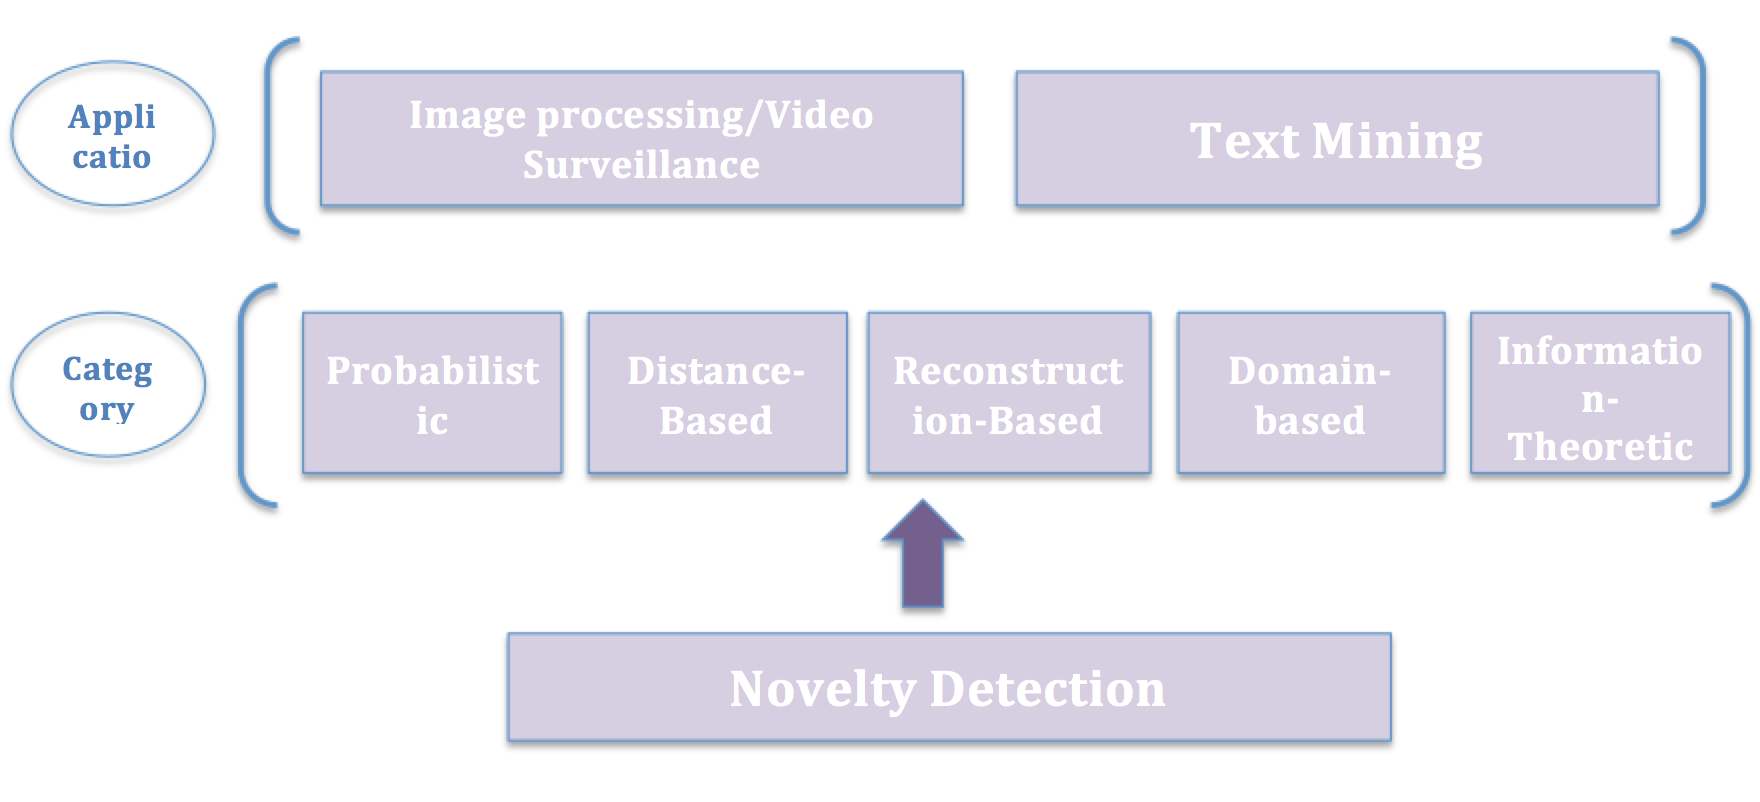
\includegraphics[width=0.5\textwidth]{33.png}
\caption{\label{} Graphical representation of the five categories with the basic two application in this survey
}
\end{figure}

\subsubsection{probabilistic}

Probabilistic approach is to estimate the obstetric probability density of data in Novelty detection. The resulting threshold to define the boundaries of the data is normal or not and test it to see whether it comes from the same distribution or not. For instance,  probabilistic methods include density of the "normal" category and the methods in training test assume that the low-density area point out of low probability of "normal" category in that area. That is a well-established field \cite{chow1970optimum}, and these methods fall into parametric and non-parametric approaches \cite{pimentel2014review}. 

\subsubsection{Distance-Based}


Distance-based methods involve the idea of nearest- neighbor or clustering analysis which is based on distance metrics between two data point. One of the most common methods used for Novelty detection is nearest neighbor-based that is assuming the normal data in training set have tightly clustered, while the novel data are located far from their nearest neighbors \cite{ismo2004outlier}.

Many distance metrics are well-defined to count the distance between two data \cite{duda2001pattern} which can be divided into distance-based methods that are the distance to kth nearest neighbor \cite{zhang2006detecting} and local density-based methods that are the distance considering the average of the k nearest neighbors \cite{ismo2004outlier}. These methods are not deal efficiently with high-dimensional. Therefore, the recent high-dimensional detection use more efficient method such as outliers detected by checking sparse sub-spaces.


Clustering-based methods contain methods like k-means clustering of distance-based novelty detection. The normal category described by the small number of prototype points in the data, and the smallest distance used to quantify abnormal.  The k-means clustering algorithm use different approaches to provide prototype locations, and it is popular in clustering structured data because of simplicity for implementation \cite{srivastava2005discovering} \cite{srivastava2006enabling}. 


\subsubsection{Reconstruction-Based}



Reconstruction-based methods are always used in regular classification problems or regression model. In the training set, reconstruction error between the actual value and the regression when mapping the abnormal data that give high novelty score. For example, neural networks can be trained in this way and can give same advantages for novelty detection.

% i may write here about neural network and Subspace-based if i need 

\subsubsection{domain-based}


This method the domain- based describe a domain that have normal data in training set. That is by realizing a boundary around the normal category, and it may not obtain a distribution in the high-density area. Domain-based methods are not sensitive to the specific density of the domain because they characterize the domain and not the class density. 





\subsubsection{Information-Theoretic Techniques}

Information-theoretic techniques compute the information content by using information-theoretic measures in the training set like entropy. The main goal is to assume novel data alter the information content in the normal data set, and calculate the metrics from the data set. Then, in the metric, find the biggest difference for the subset of a point that removed from that dataset, so this subset assumed to composed of novelty detection data. 

\subsection {Application Domain in Novelty Detection }

The application domains in novelty detection methods for the previous five categories is important in the application that contains a big data set gained from critical systems. There are six main domains of application which are electronic IT security, healthcare informatics/medical diagnostics,  industrial monitoring/damage detection, image processing/video surveillance, text mining, and sensor networks as shown in figure 4. There are some Other domains of application such as speech recognition, mobile robotics, astronomical data analysis, and environmental monitoring. Here is the two basic application in our survey which are image and text and it is a challenge.   

\begin{figure}[h!]
\centering
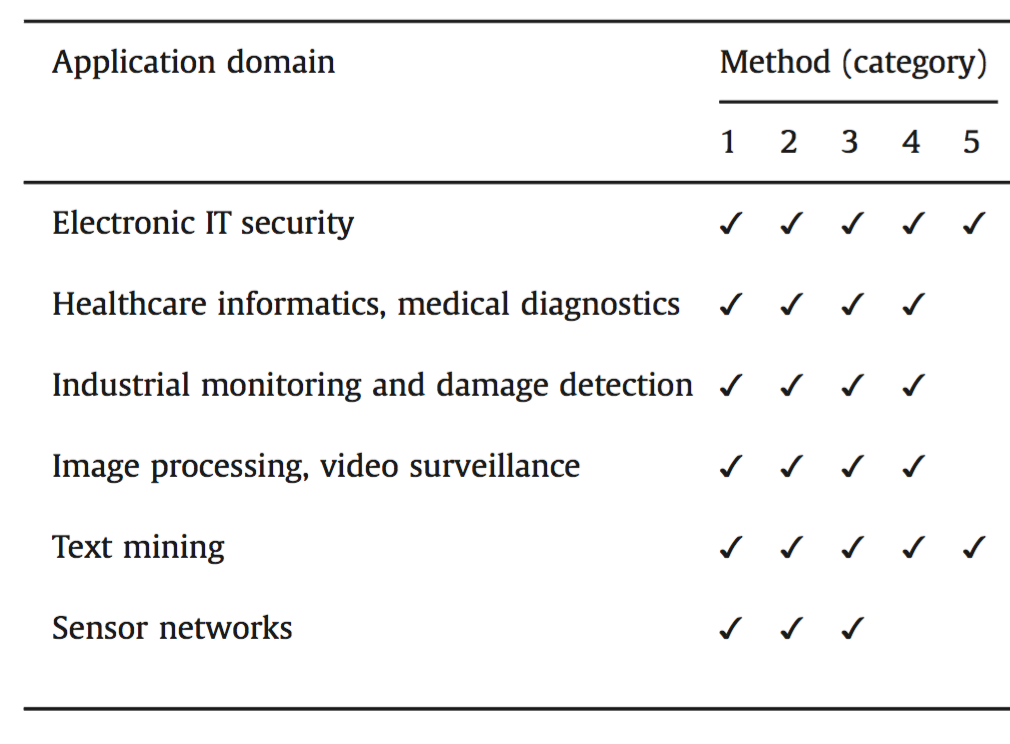
\includegraphics[width=0.4\textwidth]{22.png}
\caption{\label{}   Examples of novelty detection methods in the six main domains of application adopted by \cite{pimentel2014review} }
\end{figure}




\subsubsection{Image processing/Video Surveillance}

In image and video, the Novelty detection has been used in recognizing novel largely. For instance, extract novel data from a video stream has become concern many researchers because of a large amount of data in video accessible. Novelty detection in surveillance applications and images are an important task in order to detect videos and image that is not important. Also, anomaly detection is dealing with image motion processing or a static image. This include digit recognition \cite{lecun1990handwritten}, mammographic image analysis \cite{spence2001detection}, and video surveillance \cite{yeung2002parzen}. So the data has space, and every data contain attributes like lightness, color, or texture because the anomalies are caused by motion. The basic challenge here is that the large size of the input and online anomaly detection require with the video data \cite{chandola2009anomaly}. References for image processing and video surveillance are

\cite{pokrajac2007incremental}
\cite{ramezani2008fast}
\cite{singh2004approach}
\cite{markou2006neural}
\cite{yong2012novelty}
\cite{yong2013wildlife}

\subsubsection{ Text Mining}

The novelty detection used in text data attempt to automatic means of novelty detection. The data consider sparse, high-dimensional, and include bag-of-word features that come from advanced linguistic representations. Also, anomaly detection detects novel in a collection of documents in high dimensional and sparse. A challenge in this domain is to control the vast difference in documents belonging to one category. References for text mining are
\cite{ando2007clustering}
\cite{ertoz2004finding}
\cite{manevitz2007one}
\cite{zhuang2006parameter}
\cite{zhang2005probabilistic}
\cite{basu2004probabilistic}
 
\section{Discussion of the problems }

Advantages of context novelty detection allow a natural definition of abnormality while the disadvantages are usable only when a context can be defined \cite{chandola2009anomaly}. However, there is some problem in open set classification such as see a new word, miss spelling words, or the proper noun like names. 

%problems like 
%new word
%miss spelling
%proper noun 9( names)



\section{Conclusion }

In this paper research, we show that a few studies about the open classification for text and vision. We provide an overview of the related terms such as Novelty detection and outlier detection. We demonstrate methods of novelty detection. In the future work, we will write about the CAP model for text classification in order to find a solution for open world problem in text classification. The CAP model has two categories the distance and probability-based technique.  
 
\begin{thebibliography}
\end{thebibliography}
\bibliographystyle{IEEEtran}
\bibliography{suad}

\end{document}